%%%%%%%%%%%%%%%%%%%%%%%%%%%%%%%%%%%%%%%%%%%%%%%%%%%%%%%%%%%%%%%%%%%%%%%%%
% Template for a classical article
%%%%%%%%%%%%%%%%%%%%%%%%%%%%%%%%%%%%%%%%%%%%%%%%%%%%%%%%%%%%%%%%%%%%%%%%%
\documentclass[12pt,a4paper,notitlepage,onecolumn]{article}
\usepackage[margin=2.8cm]{geometry}
%%%%%%%%%%%%%%%%%%%%%%%%%%%%%%%%%%%%%%%%%%%%%%%%%%%%%%%%%%%%%%%%%%%%%%%%%
\newcommand{\Author}{Fabio Zanini}
\newcommand{\Title}{Exploring biomedical data}
\newcommand{\Keywords}{{data science}, {biology}}
%%%%%%%%%%%%%%%%%%%%%%%%%%%%%%%%%%%%%%%%%%%%%%%%%%%%%%%%%%%%%%%%%%%%%%%%%
\usepackage[english]{babel}
\usepackage[utf8x]{inputenc}
\usepackage{amsmath,amsfonts,amssymb,eucal,eurosym}
\usepackage{xcolor}
\usepackage{graphicx}
\usepackage[font=small, format=hang, labelfont={sf,bf}, figurename=Fig.]{caption}
%\usepackage{cite}
%\usepackage{multirow}
\usepackage{multicol}
\usepackage[colorlinks,linkcolor=red,citecolor=red]{hyperref}
\hypersetup{pdfauthor={\Author}, pdftitle={\Title}, pdfkeywords={\Keywords}}
%%%%%%%%%%%%%%%%%%%%%%%%%%%%%%%%%%%%%%%%%%%%%%%%%%%%%%%%%%%%%%%%%%%%%%%%%
\graphicspath{{./figures/}}
%%%%%%%%%%%%%%%%%%%%%%%%%%%%%%%%%%%%%%%%%%%%%%%%%%%%%%%%%%%%%%%%%%%%%%%%%
%\DeclareMathOperator\de{d\!}
%\newcommand{\comment}[1]{\textit{\textcolor{red}{#1}}}
%%%%%%%%%%%%%%%%%%%%%%%%%%%%%%%%%%%%%%%%%%%%%%%%%%%%%%%%%%%%%%%%%%%%%%%%%
\title{\Title}
\author{\Author \\[2ex] \url{http://fabilab.org}}
\date{\today}
%%%%%%%%%%%%%%%%%%%%%%%%%%%%%%%%%%%%%%%%%%%%%%%%%%%%%%%%%%%%%%%%%%%%%%%%%
\begin{document}
%%%%%%%%%%%%%%%%%%%%%%%%%%%%%%%%%%%%%%%%%%%%%%%%%%%%%%%%%%%%%%%%%%%%%%%%%
\maketitle

\section{Introduction to biomedical data exploration}
Biological and medical research is undergoing a revolution: the rise of data analytics. Traditionally, advancements in these sciences has been driven by complex and laborious experiments, each providing a little bit of evidence in support of a certain theory. String together enough of these experiments and the explanation behind them would acquire solidity and, eventually, acceptance. Scientific papers are the epitome of this style of research: a carefully crafted storyline is weaved through a few figures and figure panels, each containing one experiment with its little piece of the puzzle. Over the last few decades, however, another modus operandi has been established: large-scale experiments are conducted without specific hypotheses and are followed by (i) extensive data analytics, which generates and sometimes probes hypotheses; and (ii) smaller-scale, specific follow-up experiments that verify (or falsify) them. One key methodological difference of this new approach is the reliance on massively parallel data acquisition technologies, especially next-generation sequencing. Nowadays, as a consequence of this paradigm shift, the supply of biomedical data often exceeds the analytical skills of many biomedical researchers. If you are such a researcher and strive to adapt, this book is for you.

\subsection*{An example}
Let's imagine you are interested in a certain human gene, Itgb1. You know it encodes for a particular type of integrins, which are membrane proteins that help cells adhere to the extracellular matrix. You suspect this gene might be involved in cancer metastsis, perhaps helping the cell to leave its original location and reaching other parts of the body. A traditional approach to this -- purely fictitious -- research question would start by screening the library (or Google Scholar, or NCBI's PubMed) for papers on this topic, talking to leading experts, and thereby constructing a hypothesis of how this phenomenon might happen. Then, you would plan and conduct detailed experiments that could prove (or disprove) your hypothesis, for instance cell migration assays, knockdown and overexpression, chemical inhibition, tumor transplants in rodents, etc. Because this work is extremely time consuming, you better have a good hypothesis!

Here's an alternative plan. First, you screen a cell atlas to understand which cell types in the body express the gene. Second, you write a quick and dirty computer script to check if those cell types share any common feature. Third, you download and query a gene regulation database for transcription factors that might regulate this gene. Fourth, you explore a protein-protein interaction database to check its binding partners. Fifth, you query an online cancer mutational database to see if this gene or any of its regulators or binding partners are known oncogenes or tumor suppressors. Sixth, you query a gene ontology database to understand what pathways this gene is involved in. Seventh, remembering that cancer sometimes corrupts developmental gene programs, you download and inspect an embryonic single cell dataset focusing on actively proliferating or differentiating cells. Eighth, you browse the protein atlas to take a look at typical hystologies and fluorescent stains from this protein in various tissues and disease conditions. After all this, you construct an hypothesis and set out to verify it experimentally. You haven't even touched the literature at all.

The second plan might look absurd to you. After all, why wouldn't we check in the literature what others have found before us? Of course, if that's your concern, you are right. This example is not aiming to tell you the exact steps you should follow to discover the secret of malignancy, but rather to demonstrate how much further than the established literature you can reach if you have some understanding and skills in data exploration. This book is not about prohibiting you to use traditional methods, but there's so much more you can do to help you constructing hypotheses!

\subsection*{What this book is not}
Before proceeding any further, it is important to clarify a few expectations with our reader, lest they grow disappointed in the outcome of their efforts. In this book, I do not:

\begin{itemize}
\item promise you can learn biomedical data exploration quickly and/or without significant effort. Sorry about that: in fact, I can promise you the opposite, that if you are to succeed it will take months of dedication. But that need not be a negative thing, because people tend to like what they get better at. Enjoy the ride, its lows and its highs.
\item give you a complete list of topics you need to master to become a data explorer. Much like geographical exploration, data exploration requires some training and a fair bit of practice.
\item teach you the details of every tool mentioned. Not that I don't like tools, but the research horizon is so dynamic that they age fast. Search the internet for details.
\end{itemize}

\subsection*{Book structure}
The book is composed of two main parts:
\begin{itemize}
\item \textbf{One-year training plan:} This part gives a training plan that a newcomer in biomedical data eploration can follow to upskill from scratch. This is just a rough outline, the most important element of which is the tieline of the various steps. This timeline can be useful to adjust expectations, especially when learning hard skills such as coding that tend to distract one's mind from the overall goal.
\item \textbf{Tips, tricks, and tools:} This part includes a list of mental archetypes and sometimes practical tips that are helpful to remember and not immediately obvious to new data explorers. It might take a long time to become familiar with all these points to the point that you think of them in your daily routine, and that's just fine: more advanced readers might find them useful for inspiration or to fill knowledge gaps.
\end{itemize}


%%%%%%%%%%%%%%%%%%%%%%%%%%%%%%%%%%%%%%%%%%%%%%%%%%%%%%%%%%%%%%%%%%%%%%%%%%%%%%
\section{One-year training plan}
%%%%%%%%%%%%%%%%%%%%%%%%%%%%%%%%%%%%%%%%%%%%%%%%%%%%%%%%%%%%%%%%%%%%%%%%%%%%%%
This part contains a year long training plan to learn biomedical data analysis from scratch. I will assume that you are already familiar with experimental biological research, e.g. pipetting, running a DNA extraction, polymerase chain reaction (PCR), perhaps tissue culture and microscopy. Not that you will need those wet lab skills in the following; but I will use those contexts for illustrative purposes.

\subsection{The seascape of data exploration}
\begin{figure}
\begin{center}
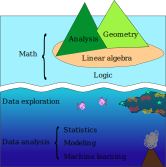
\includegraphics[width=0.5\linewidth]{island.pdf}
\caption{Island and seascape analogy of math and data science. Data exploration is similar to snorkeling in that it can be learned and enjoyed by beginners, while data analysis is more akin to scuba diving, requiring additional mathematical and computer science skills such as statistics, parametric modelling, and machine learning. Of course, some things can only be seen at depth!}
\label{fig:island}
\end{center}
\end{figure}
My college teacher, Pino Vigna, used an image to explain math: a remote island in the middle of the ocean. The beach represents linear algebra, a well established and relatively accessible topic, while functional analysis and geometry are the two mountain peaks that require training and careful planning to be conquered. (Many of you might be thinking that linear algebra is not accessible at all. I hear you! Alas, in my experience that has more to do with bad teachers than with intrinsic difficulties of the topic.) The sea surface represents logic, the very foundations of mathematical and more generally rational human thinking.

That analogy is useful for us, ambitious data explorers, as well. While math is a pure construction reaching up in the sky like a monutain island, touching the terse heights of elegance and self-consistency, however, data science is a liquid mass deeply rooted in raw biophysical measurements: the ocean itself. At the top of the water column, right below the shiny surface of logic, lies data exploration. Deeper below, where the light of ``common sense'' starts to fail, lies another kind of science, called \textit{data analysis}. Unlike exploration, analysis relies on additonal tools such as statistics, parametric modelling (e.g. differential equations) and machine learning to draw conclusions that are completely invisible to the naked eye. To keep the diving metaphor, imagine scuba diving: it's possible, but quite a bit more demanding than putting on a mask and a pair of fins. Although useful in a number of situations, we will not dwell on such topics in this book and snorkel in comfortably shallow waters. The overarching idea of this book is that even though some endeavours require deep scuba equipment, a lot of biomedical science can be done with the primitive tools of exploration: a little coding, a little stats, some intuition, basic arithmetic, and order-of-magnitude calculations.

\subsection{The first month: scientific coding} \label{ssec:firstmonth}

\begin{figure}[h]
\begin{center}
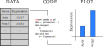
\includegraphics[width=0.8\linewidth]{parsing_csv.pdf}
\caption{Example of beginner-level scientific coding: parsing a CSV data table on gene expression and making a bar plot.}
\label{fig:parsecsv}
\end{center}
\end{figure}

I'm sorry to break you the news: exploring biomedical data will require you to talk to computers. The bad news is that computers are not particularly versed in English and much prefer stiff, unintuitive dialects called programming and scripting languages. The good news is that computers are excellent listeners and tireless helpers. Best of all, they are excellent at repetitive tasks, which is exactly what is most boring for us humans.

\subsubsection{Learning scientific coding}
This is the first thing you should do in your data exploration training. Here's some Q\&A to help you navigate these first weeks.

\paragraph{Which programming language?} I've been using mostly \textbf{Python} for a decade or so and I recommend it. It's not perfect, but it's better than most other languages for our purposes: R, matlab, bash, Perl, JavaScript, or Julia. If you know another programming language, especially among those, you'll find Python quite accessible. In any case, data exploration requires more than one machine language anyway, so this is just a way to wet your feet. A general rule would be to learn Python unless you have a close mentor who can uses a different language and offers to help you on a daily basis: then learn her/his language.
\paragraph{What kind of programming course?} Unsurprisingly, most programing classes have a very different focus from biomedical data exploration: we are niche. Instead, high-quality online resources are geared towards (i) making websites; (ii) software engineering, with emphasis on structural language constructs (e.g. functions, data types); or (iii) business analytics, especially database and user data crunching. The third kind of courses are more in line with our goals, but often require a little bit of structural knowledge to get started. I recommend you follow both a basic structural course and a basic data course. You can ignore web programming skills. Here are a few online courses (data-oriented in blue, structure-oriented in pink):

\begin{itemize}
\item \href{https://www.kaggle.com/learn/python}{\textcolor{magenta}{Kaggle: Python 3}}: a classic
\item \href{https://www.codecademy.com/learn/learn-python-3}{\textcolor{magenta}{Code Academy: Python 3}}: another classic, if not free anymore
\item \href{https://www.coursera.org/specializations/python}{\textcolor{magenta}{Coursera: Python for everybody (U Michigan)}}: good if you prefer a structured course
\item \href{https://www.kaggle.com/learn/data-visualization}{\textcolor{magenta}{Kaggle: Data visualization}}: focused on data plotting makes it a little specific, but most new explorers find motivation in charts, which is good
\item \href{https://www.codecademy.com/learn/paths/analyze-data-with-python}{\textcolor{blue}{Code Academy: Analyze data with Python}}
\item \href{https://pythonforbiologists.com/}{\textcolor{blue}{Martin Jones' Python for Biologists}}: this one is a book (now three books) that has accompanied many a biologist learning data exploration before. I personally don't enjoy too much learning coding from printed sheets of dead trees, so I'd rather use the PDF version. They offer classes too.
\item \href{http://fabilab.org/pages/teaching.html}{\textcolor{blue}{My own lecture slides}}: a little terse, students find them useful as a cheatsheet alongside a proper course
\end{itemize}

\paragraph{How much should learn every day?} As much as you can. In this first month, learning coding is the number one priority, so focus on that. Ideally you'd spend 8 hours learning coding every day. You might think that's too much, but learning new things is quite hard on our memory, and keeping a fast pace for a few weeks appears to be an effective way to overcome that barrier.

\paragraph{I see all these packages, which ones do I actually need to install?} More in the \nameref{sec:tips} section, but for sure you'll need:

\begin{itemize}
\item numpy: \url{https://numpy.org/}
\item scipy: \url{https://www.scipy.org/}
\item pandas: \url{https://pandas.pydata.org/}
\item matplotlib: \url{https://matplotlib.org/}
\item seaborn: \url{https://seaborn.pydata.org/}
\item Biopython: \url{https://biopython.org/}
\end{itemize}

Installing packages is explained in the \nameref{sec:tips} section too.

\paragraph{How good do I need to become?} Good enough that you are not overwhelmed by the coding when looking at biomedical data and can spare a small fraction of your brain power to actually think of the science. It's a gradual process, of course. When the following sentences start making sense to you and you can actually do (or imagine yourself doing) them, you are good enough to start snorkeling:

\begin{itemize}
\item Parse a CSV with gene expression data and find the highest expressed gene.
\item Read in the spreadsheet and make a scatter plot of the first two colunms.
\item Find an amino acid motif (e.g. GGKG) in a protein sequence from a Fasta file.
\end{itemize}

By the time you are done with this step, you should be able to uderstand the code in Figure~\ref{fig:parsecsv} and do the same on a data table of yours.

\subsubsection{Structure of an explorer's projects folder}
\begin{figure}
\begin{center}
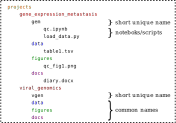
\includegraphics[width=0.7\linewidth]{folder_org.pdf}
\caption{Typical organisation of a projects folder.}
\label{fig:projorg}
\end{center}
\end{figure}
As you start your coding forays, you will wonder where to store your code, data, and results. Figure~\ref{fig:projorg} is the structure I recommend using (and the one I use myself). First, make a \textit{projects} folder on your computer (or whatever other name you fancy). Inside, make a different folder for each project or exploration you are working on. Imagine each project is a different reef you want to snorkel at, then your folder contains all the info required to find the place, the dangers, the tools you need, etc. Inside each project folder there are a few subfolders:

\begin{itemize}
\item \textbf{data:} It includes raw data that are needed by your code and processed data that are produced by the code itself. It might contain other people's data in addition to yours, e.g. from public databases.
\item \textbf{figures:} It contains chart, plots, and figures that are produced by your exploration. The reason for this folder is that a picture is worth a thousand words, so explaining your results to collaborators or teammates is much easier if you know where to find your figures.
\item \textbf{docs:} Contains papers on the topic which you found during your literature searches, as well as your explorer's diary (see below).
\item \textbf{code folder:} This folder contains the code for your explorations. The folder name should not be ``code folder'', but rather a short, unique name without spaces (see examples in Figure~\ref{fig:projorg}). The reason for this naming choice has to do with Python modules and will become clear later on.
\end{itemize}

Beyond this basic structure, organising each of these folders with subfolders if needed is a good idea.

\subsubsection{Keeping an explorer diary}
As any lab researcher can attest, it is key to keep records of what you have been doing in a lab book so you can reconstruct your actions when things go wrong (or, more rarely, go well!). Same goes for your computational projects: there is great benefit in keeping track of your explorations.

The important tip here is that your code and the rest of the project are generally tracked separately. We will see later on how to track code properly, so don't worry about it for now. To track the project in general, the minimal requirement is a file in the \textit{docs} folder, called ``diary'' or similar, that you fill in every time you have some notes or progress. Even a short paragraph with a date and describing what you have been coding today is a great way of recording progress: no need to spend 2 hours each day writing diary.

The format of such diary is quite free. I just use text or docx files, or Google documents. There are electronic notebooks such as labarchives (\url{https://www.labarchives.com/}) and benchling (\url{https://www.benchling.com/}). Some people find these convenient, but personally I prefer a simple file in each project folder, because I always have it with me and can decide the format completely. Unlike paper lab books and diaries, it's very easy to make a copy of a file and carry it with your into your new job when the time comes. With online services, you will have to figure out how to migrate the data out and that is usually a headache.


\subsection{The first quarter: learn to ask questions}
As you become more familiar with scientific coding over the first weeks, you can start taking a look at a data set of yours. At this stage, it is important that the data set you choose is something you really care about, not just a toy data table as you have learned in your online courses.

The goal for these two months is \textbf{learning how to ask the right questions} about the data, and how to phrase those questions to a human and a computer alike. This might sound silly: we want answers, not questions, right? Well that's correct, of course. At the same time, in data exploration, formulating reasonable hypotheses is as important as verifying them. Indeed, hypothesis generation rooted in data as opposed to just pure intuition is one of the main advantages of data exploration in the first place.

\paragraph{Example: Gene expression data.} Imagine you have collected RNA-Seq or other gene expression data on your disease of interest, say cancer. You have 2 biological replicate samples from healthy controls, and 2 from sick people. Of course, your ultimate goal is to understand the causes and processes of cancer biology, but that question is too broad to be answered directly. Instead, it is necessary to learn to formulate precise questions that \textit{can} be answered, and then refine and steer them towards that final goal. Here's a few questions that would be useful as a start:

\begin{itemize}
\item What is the highest expressed gene across all samples?
\item What is the sum of expression of all genes in the 4 samples?
\item What are the \textit{measurement units} for these numbers?
\item What is the expression of housekeeping genes that should \textit{not} differ between healthy and cancer subjects?
\item What are the main sources of difference between any two samples?
\item What is the expression of genes known to be altered in this type of cancer?
\end{itemize}

All these questions are not directly asking the final question, which is usually: \textit{What are the genes that are upregulated and downregulated in cancer?} The best answer to that question lies outside the realm of data exploration and involves quite accurate knowledge and use of statistics. In fact, there is computer software (e.g. edgeR: \url{https://academic.oup.com/bioinformatics/article-lookup/doi/10.1093/bioinformatics/btp616}) that is designed exactly to answer that question. Nonetheless, those primitive questions can be extremely useful to understand the general context of the data, to check for problems in the data collection, to prompt further investigations, and to double check that the results from a statistical analysis make sense. The target of these two months is to be able to ask and answer a number of those questions yourself.

Here is a list of useful notions that one should become aware during this time.

\paragraph{Night science:} Bad hypotheses can result in wasting years of your life, and good hypotheses don't grow on trees. Instead, the practice of generating and recognizing promising hypotheses is a skill that requires training:

\begin{itemize}
\item {\footnotesize \url{https://genomebiology.biomedcentral.com/articles/10.1186/s13059-019-1800-6}}
\item {\footnotesize \url{https://genomebiology.biomedcentral.com/articles/10.1186/s13059-020-02133-w}}
\end{itemize}

\begin{figure}
\begin{center}
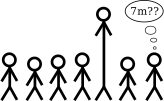
\includegraphics[width=0.4\linewidth]{7m.pdf}
\caption{Sanity checks are an essential first step in data exploration. If one of your study participants is reported to be 7~m tall, your data is probably corrupt and you need to do something about it \textit{now}.}
\label{fig:7m}
\end{center}
\end{figure}


\paragraph{Sanity checks/QC:} Biomedical experiments happen in extremely well controlled contexts: you don't just go to the lab, pick up a pipette, and start transferring random liquids from one tube to another. When looking at data for the first time, it is important to ask questions about a number of boring but expected patterns. For instance, if you are counting cells through a FACS machine, you should have an expectation about their rough numbers, whether they are a thousand or a million. When looking at genome sequences, you expect there to be only four letters, namely A, C, G, and T. When looking at patient weight, height, BMI, and other similar measurements, you expect most people to fall into fairly tight ranges around the population average. If someone is reported as being 7~m tall, your data is probably corrupted and you need to fix this problem before moving on with your exploration. These initial questions on the data, also called quality check (QC), are important to establish credibility in the data acquisition pipeline, and to make you familiar with the strong and weak aspects of the data. There's no real limit as to how many such questions you should ask, but generally a thorough QC saves you a lot of trouble later on.

\paragraph{Units of measurement:} Gene expression in RNA-Seq is measured in ``number of sequencing reads''. This means: you sequence a bunch of DNA molecules, and then count them. Learning to recognize and manipulate the units of biophysical measurements our data is generated by is an essential, yet virtually untaught skill in biomedicine:

\begin{itemize}
\item  TODO (sigh!)
\end{itemize}

\paragraph{Orders of magnitude:} This point is related to the previous one about units. Data exploration often involves quantitative measurements and numbers, and it is important to develop as of the expected orders of magnitude for numerical data. I already mentioned as an example that during a cell sorting (FACS) experiment you should know whether 1,000 or 1~million cells are expected; the same idea applies to most numbers you see in your data:

\begin{itemize}
\item In RNA-Seq, you might find that your data table has 60,000 genes: is that reasonable? Upon further inspection, most of them have exactly zero detected reads and only 3,000 are positive: is \textit{this} reasonable and expected? RNA-Seq is very noisy for low-expressed genes and you wonder why that is, so it's useful to ask youself: how many \textit{mRNA molecules} for this gene are there in my sample? Of course, if the entire sample contained a single molecule in average, you expect a lot more noise than if the sample contained 100.
\item Another example from genomics: you perform a ChIP-Seq experiment to find the binding sites of a certain transctiption factor across the human genome, and you find 3 binding sites. Is this a high or low number? What order of magnitude were you expecting?
\item A third example on viral evolution. RNA viruses such as SARS-CoV2 usually mutate quite rapidly, perhaps once every 100,000 copies. They also produce a huge number of viruses inside the body upon infection, perhaps billions. So do you expect to see mutants arising during an infection? Is it surprising that new variants of this virus emerge?
\end{itemize}

\paragraph{Start specific, expand by repetition:} In the first month, you learned basic scientific programming. Now it's time to start using those skills to answer questions about your data. At first, looking at data can be overwhelming: there are so many questions that could be asked! That's normal, so don't worry. A good strategy out of that mental blockade is to divide the problem in two parts: (i) Start with a simple and very well defined question (e.g. ``what is the highest expressed gene in a certain sample?'') and write a piece of code to find the answer; (ii) Expand from that question to closely related ones that include some element of repetition (e.g. ``what is the highest expressed gene in \textit{each} sample''), and code the answer by expandinng your previous code and using one or two \textit{for} loops (and, if you want, functions). This pattern of ``start specific and simple, and expand by repetition'' is important because you'll be using it all the time in your future explorations. Because computers are so good at repetitive tasks, it leverages one of the essential reasons to prefer them to manual data inspection on, say, a printed piece of paper. If you are trying to exercise this step and find yourself wondering what a for loop is, go back now to your online courses or google your doubts now and make sure you understand how it works and how to use it.


\begin{figure}
\begin{center}
\includegraphics[width=0.7\linewidth]{Visualisations}
\caption{Try out several visualisations for the same data and you'll be surprised how some convey your message much more easily than others. From top left and clockwise: line plot, scatter plot, bar plot, table, pie chart, heatmap.}
\label{fig:viz}
\end{center}
\end{figure}
\paragraph{Two plots are better than one:} By now you should have some familiarity with plotting (usually with matplotlib). When snorkeling data, it is often unclear which one is the best way to visualise the result of the exploration. Among other options (see Figure~\ref{fig:viz}):

\begin{itemize}
\item line plots
\item scatter plots
\item heatmaps
\item bar plots
\item violin plots (aka kernel density estimates or KDE)
\item swarm plots
\item pie charts
\item tables
\item area plots
\end{itemize}

There is no general recommendation here, it really depends on the data. The important point, at this stage, is that trying out a few visualisations instead of just one can turn out really useful. So before you copy-paste a figure into your next presentation, try out a few alternatives and see which one makes it easiest to understand your result.

\subsubsection{Terminal basics}
TODO


\subsection{The first semester: tracking, recycling, and polishing}
In your first month, section~\ref{ssec:firstmonth}, you learned to organise your \textit{projects} folder. You also learned to keep an explorer's diary with your progress updates. We are going to revisit that idea here, but covering the two points we left hanging: (i) how to track code and (ii) why the code folder in each project needs a short, unique name.

\subsubsection{Code versioning with git}
One of the key advantages of data exploration over wet lab experiments is that you can run variations of your explorations quite easily by tweaking your code a little. In many cases, these variations also run at no monetary cost. That benefit comes with a risk. If you tweak the code a lot of times - which you should, and you will - you risk to lose track of what version of the code worked well and produced useful results. Perhaps needless to say, you cannot publish the result of an exploration that not even you know how to run anymore. To avoid variation-linked loss of knowledge, beginners often copy-paste files containing scripts or notebooks and give them slightly different names, e.g. ``analysis\_version1'', ``analysis\_version2'', and so on. That's better than forgetting, but nowadays there is a more effective method: version control systems (VCS).

Git (\url{https://git-scm.com/}) is the most widepreas VCS and a key tool to update your code without the risk of forgetting. It basically keeps a history of your code folder, as detailed as you care for it to be, and lets you freely travel back in time to previous versions, recover code you have deleted in the meanwhile, and paste it right back on top of the latest revision. See the section \ref{sec:tips} for more info and links.

Each of your project folder can be converted into a git repository by just going inside the folder and running ``git init''. You then have to decide which files you want to track. Generally you want to track at least the whole code folder inside your project. It is a good idea to commit small and commit often, that is to make a lot of versions. The more versions you have, the easier it is to go back to exactly the version you need.

It is convenient to create a new file inside the same folder with a special name: ``.gitignore'' (yes, it starts with a dot, and no caps). This file contains a list of folders, files, or file patterns that you want to ignore, such that git will not track them. You might wonder: why do I want to exclude files from tracking? Well there are two main kinds of things you want to exclude:

\begin{enumerate}
\item \textbf{computer-generated cache:} For instance, Python sometimes will create folders called ``\_\_pycache\_\_'' (yes, starting and ending with a double underscore) or files that end in ``.pyb''. You don't need to track those files because your computer can easily regenerate them automatically.
\item \textbf{large data files:} Git (and all VCS) does not work well with large data files. One reason is that if you have a large file (e.g. 1~GB) and it changes 100 times, you need 100~GB of disk space to store all historical versions of this file. So large data files should be added to your .gitignore. In fact, I often either (i) ignore the whole \textit{data} folder, or (ii) create a subfolder in \textit{data} called ``raw'' or ``big'' and ignore that.
\end{enumerate}

Atlassian has a good guide to .gitignore patterns at \url{https://www.atlassian.com/git/tutorials/saving-changes/gitignore}. The official docs are also somewhat useful at \url{https://git-scm.com/docs/gitignore}.

Remember: if you use git correctly, you will \textit{never} be afraid to delete files or make code changes again.

\subsubsection{Recycling code across scopes}
The second skill we need to learn within the first six months is to recycle pieces of code you have already written. This is a point which is lost on most self-taught data explorers, so if you are one, you might want to read on.

\paragraph{Example: data ingestion.} Imagine you have a block of code, perhaps 30 lines or so, that reads some gene expression data and processes it lightly, for instance normalising the numbers to some total, renaming samples according to some rules, and adding some metadata such as subject age and sex. (This kind of operation is common enough to deserve a name, data ingestion.) Although you perform many different types of explorations on the same data, this block of code is likely to be the same for all of them. Your first instinct might be to just copy-paste the block into each one of your notebooks. That works at the start and you end up with 15 notebooks, all with that block at the top. Problems come when you need to change the block a little, e.g. to make space for another sample or a second data set. Now because your code is scattered around all those files, you need to modify each and every one of them! That'll take you an hour and if there is a typo you have to start all over again\dots not really ideal. It would be much easier to have a data ingestion function in a separate file and just \textit{use} it in all notebooks.

\paragraph{Example: color palettes.} When you disseminate the results of your explorations, e.g. in a scientific paper or a conference poster, graphics and colors are quite important. Humans have a hyper-performant visual cortex and are extremely sensitive to graphic content, therefore you should combine colors that fit together harmoniously rather than just cyan, magenta, and some awful lawn-green. How do you find a good color palette? By trying out a few, obviously. Now if your figures are generated by 7 different notebooks (mine usually are), you need to change colors in each notebook every time you want to try out a new palette. You would save 85\% of your time if you had a single file containing the palette and recycled it in every notebook.

Code recycling depends a little on the programming language you choose. For Python, it hinges on two separate mechanisms, functions and modules. It's time for you to start using both.

\paragraph{Functions:} You should have seen how to write a Python function in your first month. If not, now it's a good time to go online and figure that out. So the first step towards code recycling is taking the block of code you use a lot and wrap it in a function. If you haven't used functions a lot in the past, you'll need to think quite a bit about I/O, i.e. what arguments you need (input), what your function \textit{returns} (output), and what your function \textit{modifies} in place (side effects). There is not a single, correct way to encapsulate your code into a function, instead you have considerable freedom to choose options, additional arguments, data types, etc. At this stage, just try a few times and see what works best for you.

\paragraph{Modules:} A function within a notebook can only be used by that exact notebook. Therefore, functions alone are not sufficient to let you recycle code across notebooks. To achieve that, Python uses a mechanism called \textit{import}. Importing means letting the computer browse through a Python file for you, extracting a bunch of functions (and other things) you need, and making them available in the current notebook. Importing has two steps:

\begin{enumerate}
\item \textbf{Make a module:} Unfortunately, Python cannot import from a notebook, only a Python module -- a text file ending in ``.py'' (but see below if you feel corageous), so you'll have to move your function into such a file. How do you open a ``.py'' file? With a text editor (see section \ref{sec:tips}) such as sublime (\url{https://www.sublimetext.com/}). Just take the function, paste it inside that file (e.g. myfunctions.py), and save it in your code folder (within your project folder). If the function uses any imports (e.g. pandas, numpy) you need to import those at the top of your py file as well. If you are already using plain Python scripts instead of notebooks, you can skip this step, because scripts are automatically also modules (that's why I don't use notebooks myself: too much code recycling going on).
\item \textbf{Import module:} For security reasons, each Python installation keeps a whitelist of folders that you can import from, called ``PYTHONPATH''. You have to add the absolute path to the folder containing your module to the whitelist. Here is a guide on how to do that: \\ \url{http://www.bdnyc.org/2012/09/editing-pythonpath-to-import-modules/}.
\end{enumerate}


\noindent
\underline{Note on notebooks:} There seems to be a way to import from a notebook: \url{https://nbviewer.jupyter.org/github/ipython/ipython/blob/master/examples/IPython\%20Kernel/Importing\%20Notebooks.ipynb}. Feel free to try it out, though I suspect it is a few notches too difficult for most readers of this guide. My own opinion: not worth it.

\subsubsection{Polishing graphics}
\begin{figure}
\begin{center}
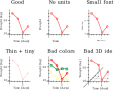
\includegraphics[width=0.81\linewidth]{visualisations2.pdf}
\caption{Common beginner mistakes for data visualisation. Polishing several aspects of the exploration figures indicates proficiency and maturity.}
\label{fig:viz2}
\end{center}
\end{figure}
Figures are an essential component of scientific dissemination, so it's important to know how to make effective ones. You'll be surprised by how much difference a better font size, color palette, and data representation makes. Making figures for data exploration is a little different from hypothesis-driven science, because the question is not set in stone. A few general rules apply (see also Figure~\ref{fig:viz2}):

\paragraph{Axis names and units:} Whenever you show data -- not a schematic -- each axis needs a name and units of measurement. If you don't know what to put there, stop and think about it.

\paragraph{Font size and line thickness:} All text in a figure must be readable, i.e. in a big enough font. If you write labels {\tiny like this}, it is not only difficult to read: your reader will get angry and think that you're doing a poor job. Same holds for thin, thin lines: best avoided, use thicker ones.

\paragraph{Color blind people:} Yes they exist, around 8\% of the male population cannot distinguish red from green to some extent. If that person is in charge of hires and you show two curves that look the same, they'll hire someone else. Color Oracle (\url{https://colororacle.org/index.html}) can put a virtual filter on your screen to check if your plots are good.

\paragraph{Log/logit scales:} If your data is positive and spans several orders of magnitude, scaling one or both the axes to logarithmic scale might simplify the message. A similar but less well known tenet holds for data that is positive and less than 1, typically fractions (e.g. ``what fraction of my subjects is sick?'' is a number between 0 and 1). In this case, using the logit scale might help: \url{https://www.includehelp.com/python/linear-vs-log-vs-logit-scale.aspx} (fun fact: I was the one adding logit to matplotlib). If your data includes exact 0 or 1s, you should consider pseudocounts (and its logit inverse, i.e. clipping the data between say 0.0001 and 0.99999).

\paragraph{Title:} A figure with an explanatory title is more useful than one without.

\paragraph{3D plots:} Better avoided. I know, nowadays so many people are showing fancy 3D plots in Nature papers. In my experience, 3D plots are \textit{almost} never useful and in most cases make things less clear, not more. The reason is pretty clear: papers and slides, whether electronic or printed, are 2D surfaces anyway. The day virtual reality visors become the standard way to read scientific literature I'll be happy to change my mind. If you really want to use a 3D plot, at least be aware of the angle of projection: people won't see anything else.

The most difficult thing in terms of figure polishing is choosing an appropriate virualisation for the data. In fact, data visualisation is a science on its own. Given some data, should you use a scatter plot? Or lines, bars, a heatmap? Here a few links you might find useful:
 
\begin{itemize}
\item matplotlib (\url{https://matplotlib.org/}) and seaborn (\url{https://seaborn.pydata.org/})'s docs are very useful as reference pages
\item \url{https://realpython.com/pandas-plot-python/}: better than most tutorials
\item \url{https://bl.ocks.org/}: one of the best sources of inspiration for thinking about data visualisation options
\end{itemize}

Although I won't go into details here, there is one questions that should be on your mind all along as you consider options: ``Is the message clearer this way?''. Sometimes, the prettiest plots do not covery the message in the clearest way: an ugly plot might be easier to understand. In that case, I'd recommend you choose the clear plot and try to make it prettier rather than the other way around.

\paragraph{The basic workflow for polishing figures in Python:} Most Python data explorers use \textit{matplotlib} (some are aware of this fact, some aren't). In order to make a polished figure with lots of customisation, you need to focus on one matplotlib concept: the \text{axes}: \url{https://matplotlib.org/3.3.3/api/axes\_api.html}. Unfortunately, the official documentation is not very useful so I'll explain a little how to use and axes (yes, spelled with an ``e'') here. Here's how I usually make polished plots for my papers:

\begin{verbatim}
import matplotlib.pyplot as plt

# Make axes
fig, ax = plt.subplots()

# Plot data (just an example)
ax.scatter(x, y, linewidth=2, color='steelblue')

# Polish plot
ax.set_xscale('log')
ax.set_title('Data shows XYZ')
[... more options ...]
\end{verbatim}

In other words, there are three operations: (i) create an axes, (ii) plot your data in that axes, and (iii) polish the axes afterwards. Avoid using functions such as \texttt{plt.plot}, \texttt{plt.scatter}, etc. and use the axes methods with the same names (\texttt{ax.plot}, \texttt{ax.scatter}) instead.

\subsubsection{Code optimization: part 1}
As a general rule, programming languages that are easy to learn (e.g. Python, R) tend to be slower than lower-level languages (e.g. C, Fortran). Although in many explorations your laptop is fast enough, as you start nesting for loops you might find yourself waiting impatiently for your code to run. 

There are known code patterns that tend to slow down Python code, e.g.:

{\scriptsize
\begin{itemize}
\item \url{https://towardsdatascience.com/optimizing-your-python-code-156d4b8f4a29}
\item \url{https://www.analyticsvidhya.com/blog/2019/09/4-methods-optimize-python-code-data-science/}
\end{itemize}
}

\noindent
Two patterns are especially prevalent:

\paragraph{1. For loops VS vectorized code:} One reason \textit{numpy} was written is to speed up for loops. numpy is written mostly in a faster language (C), greatly speeding up your code. The price you pay is that you have to use numpy tools instead of plain for loops. Imagine you have a list of gene expressions and you want to know which ones are above 5 counts. Here's how the code would look without and with numpy:

\begin{multicols}{2}[]
\noindent
\textbf{Without numpy:}

\begin{verbatim}
result = []
for value in mylist:
    if value > 5:
        result.append(value)
\end{verbatim}

\noindent
\textbf{With numpy:}

\begin{verbatim}
myarray = np.asarray(mylist)
result = myarray[myarray > 5]


\end{verbatim}
\end{multicols}

The left code is easier to understand, right? But the right code runs perhaps 1,000 times faster. So if your exploration takes 10 minutes and is full of for loops, there is a chance it could run in 0.1 seconds if you adapted it to use numpy instead. The same argument applies to \textit{pandas}, because pandas uses numpy to crunch numbers. The kind of tricks such as the right code example are generally called \textbf{vectorized code}. Yes, it is a pain to learn, but it does help so here a few links on that:

{\scriptsize
\begin{itemize}
\item \url{https://engineering.upside.com/a-beginners-guide-to-optimizing-pandas-code-for-speed-c09ef2c6a4d6}
\item \url{https://towardsdatascience.com/python-vectorization-5b882eeef658} {\normalsize : a little mathy}
\end{itemize}
}

\begin{figure}[hb]
\begin{center}
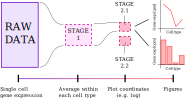
\includegraphics[width=0.8\linewidth]{datastaging.pdf}
\caption{Data staging means identifying waypoints in your exploration that make it faster and more systematic. The key feature of a stage is that later steps only depend on the waypoint processed data, not on the raw data.}
\label{fig:datastaging}
\end{center}
\end{figure}
\paragraph{2. Data staging:} Most explorations follow a certain pattern: they start from a large, raw data set and end with a small, specific set of results. In other words, the data passes through a size funnel that distills its essence and discards the ballast. Because of this gradual reduction in size, it is sometimes useful to identify waypoints that decouple the exploration into independent sections (see Figure~\ref{fig:datastaging}). As an example, think about single cell transcriptomics. In many kinds of explorations, we don't really need the gene expression of each single cell: we can cluster the cells into cell types and then average within each type. For exlorations that only rely on averages, it is best to (i) compute the averages and save them into a variable, and (ii) make the later part of the workflow reliant \textit{only} on these averages. Another classical metric in single cell transcriptomics is ``fraction of expressing cells`` within each population. Even though a cell type might have 10,000 cells, once we compute the fraction it is a single number, i.e. we save a lot of space and computing time for later analyses. This process can be called \textit{data staging}.

\noindent
\textbf{Remember:} Never spend your time optimizing code that is not a bottleneck (i.e. it is already fast enough). It's a losing game. 

\subsection{The first year: independent and live exploration, caching}
\subsubsection{Independent exploration}
The main goal for the end of 12 months of training in data exploration is deceivingly simple: basic independence. What I mean is that \textit{given a specific biomedical research question and some data}, you are able to:

\begin{itemize}
\item Read the data
\item Perform QC and sanity checks
\item Look for global patterns
\item Articulate the overall question into a series of specific, smaller questions that a computer can help you answer
\item Produce good-looking and understandable figures
\item Share your code and its history with your audience (e.g. via GitHub)
\end{itemize}

You might be thinking: ``That's a lot! Isn't that what independent researchers (e.g. postdocs, group leaders) do?'' Well, yes, but those folks, including myself, also have to (i) come up with interesting research questions and (ii) figure out how to generate or obtain the data (including how to pay for it). Nevertheless, the list is long and ambitious and you should be proud once you get there! One step at a time, you can cross America.

Given most of these topics were covered in the first six months of training, what remains to learn in the second half? Well, the second half of the year is mostly dedicated to two activities:

\begin{enumerate}
\item \textbf{Practice:} By the end of the year, your data exploration skills should be a well oiled machine. You should be able to be fluent enough that 90\% of your attention is spent on the biomedical data rather than on the skills. If you struggle parsing text files, polishing your plots, installing packages, you need more practice.
\item \textbf{Additional topics}: Although the basics are the same for all explorers, you will need specific skills beyond this book depending on your projects and interests. For instance:
\begin{itemize}
\item If you like software engineering, why don't you learn how to take an architects' perspective on data exploration?
\item If you work a lot with 3D protein structures, you probably want to upskill in Pymol (\url{https://pymol.org/2/}).\item If you deal with big data, there's no way around databases and basics of a big data language, e.g. Apache spark (\url{https://spark.apache.org/}).
\item If you need extremely fast code, you probably want to learn a lower-level programming language such as C++.
\item If you find yourself doing a lot of statistics and predictions, machine (and pehaps deep) learning is the way forward!
\end{itemize}
\end{enumerate} 

\subsubsection{Live exploration}
In the grand scheme of things, this is a secondary goal. However, people really love when I explore the data in front of their eyes, for instance during a lab meeting or a video call, so I thought I'd include this if you want to look good too.

Live data exploration has three prerequisites:
\begin{enumerate}
\item \textbf{Infrastructure:} You don't have time to write functions, look for data on your computer, figure out data formats, QC, etc. Those things must all be prepared in advance so that when the time comes, you can just run the function instead of writing it.
\item \textbf{Efficiency:} An average person can wait for your code for around 3 seconds before getting impatient, so whatever exploration you are planning to run live, it has to be faster than that. If that sounds quick, remember a modern computer can perform 9 billion operations in that time frame, so don't underestimate you laptop. However, if a certain function usually takes 30 seconds to run, you might want to optimise it a little to reduce that time. 
\item \textbf{Memory:} The 3-second waiting time includes the time it takes you to remember which function you want to use, so you're better off if you have a mental map of your explorations and functions. Every person has a different way of memorising, but for me the best way is writing files and functions with a certain regularity to them. Perhaps keeping a list of functions that you might want to run live is a good idea as well.
\end{enumerate}

Although live demonstrations can be as complex as you want them to, most of the time your coworkers will ask you to reproduce a figure you sent them. Alternatively, they might want to run the same analysis but on a slightly different part of the data (e.g. a different gene in the genome, or a different sample). Whenever you are writing a block of code (or a function) that creates a polished figure you send around, always think: could I run this on a different gene? and a different sample? In many cases, a little change in the code will add generality and make live coding a lot easier. Here's an example:

\begin{multicols}{2}[]
\textbf{Initial version:}

\begin{verbatim}
# Read file
df = pd.read_csv('myfile.tsv')

# Preprocess
df.set_index('id', inplace=True)
df['time'] /= 100.

# Extract gene expression
df_ACTB = df['ACTB']

# Print mean expression
df_ACTB_mean = df_ACTB.mean()
print(df_ACTB_mean)

\end{verbatim}

\textbf{Improved version:}

\begin{verbatim}
def read(fn='myfile.tsv'):
    df = pd.read_csv(fn)
    df.set_index('id', inplace=True)
    df['time'] /= 100.


def print_mean(data=df, gene='ACTB'):
    dfm = data[gene].mean()
    print(dfm)
    return dfm


df = read()
print_mean()
\end{verbatim}
\end{multicols}

These two codes do the same thing, but the improved version has opened a few doors:
\begin{itemize}
\item If you want to run the whole thing on a different dataset, you can just change the file name in the first function.
\item If you want to change the gene you print, you can just change the gene in the second function.
\end{itemize}

This ability to code a specific exploration while keeping your options open for side adventures, questions, and requests is a factor that distinguishes beginner explorers from proficient ones. Try to answer a concrete question, but fly your mind as high as you can in the process: that is useful for live explorations too.

\subsubsection{Data caching}
\begin{figure}[h]
\begin{center}
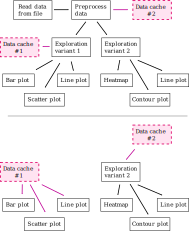
\includegraphics[width=0.6\linewidth]{datacache.pdf}
\caption{Data caching means storing a processed version of the data before different explorations diverge (e.g. right before visualisation) to save time, thereby increasing efficiency and enabling live exploration. Top: cache generation. Bottom: cache use. If you are tweaking the visualisations of exploration 1, cache 2.1 saves you the time for reading, preprocessing, and running the exploration itself. If you are tweaking exloration 2, cache 1 saves you the time for preprocessing.}
\label{fig:datacache}
\end{center}
\end{figure}
Because it lacks an initial question, data exploration grows rather organically. Many explorations share the initial part of the workflow (e.g. reading the data, preprocessing) and differ towards the end. Sometimes, the only difference is the exact visualisation chosen (e.g. bar plot or line plot).

This kind of data manipulation is well suited to \textit{data caching}. That means storing a processed version of the data right before the different explorations diverge, so that you don't need to run the first part more than once. Figure~\ref{fig:datacache} illustrates this concept. We have one data set with two explorations and three possible visualisations for each. We expect to spend a lot of time tinkering with the visualisations and possibly the exploration code itself. Without caching, every time we rerun the analysis we have to restart from the initial data file and follow all black arrows. Data caching has two steps:
\begin{enumerate}
\item \textbf{Cache generation (top):}  For exploration 1 we store a data cache right before the plotting (cache 1). Moreover, because exploration 2 is not quite stable, we set up cache 2 right before that step. 
\item \textbf{Cache use (bottom):} When we want to polish the graphics of exploration 1, we can directly load data cache 1 and save the time for preprocessing and exploration 1. A similar argument applies when we want to polish exploration 2, in which case we use cache 2.
\end{enumerate}

You might be wondering about the difference between using data caches and data stages. Like caches, stages also store a processed version of the data and you can tweak subsequent code. At a general level, stages and caches are the same thing except that variables(stages) live in volatile memory (RAM) which is deleted whenever you close your Python session, while data caches are stored on your hard drive and therefore permanent. Therefore, caches can be thought as permanent stages, or stages can be thought as volatile caches.

Here a typical piece of code corresponding to exploration 1 in Figure~\ref{fig:datacache}:

\begin{verbatim}
import os
import pandas as pd

# Check for cache 1
if os.path.isfile(file_cache1):
    # Use cache 1 if available
    result1 = pd.read_csv(file_cache1)
else:
    # Cache1 not available, check for cache 2
    if os.path.isfile(file_cache2):
        # Use cache 2 if available
        df = pd.read_csv(file_cache2)
    else:
        # No cache, follow black arrows
        df = pd.read_data(...)
        preprocess(df)

        # Generate cache 2
        df.to_csv(file_cache2)
    
    result1 = exploration1(df)

    # Generate cache 1
    result1.to_csv(file_cache1)

# Plot
plot_result(result1, kind='bar')
plot_result(result1, kind='line')
...
\end{verbatim}

%%%%%%%%%%%%%%%%%%%%%%%%%%%%%%%%%%%%%%%%%%%%%%%%%%%%%%%%%%%%%%%%%%%%%%%%%%%%%%
\newpage
\section{Tips, tricks, and tools} \label{sec:tips}
%%%%%%%%%%%%%%%%%%%%%%%%%%%%%%%%%%%%%%%%%%%%%%%%%%%%%%%%%%%%%%%%%%%%%%%%%%%%%%

\subsection{Installing Python}
One of the first obstacles for the beginner data explorer. There are a few ways to install Python and it mainly depends on what operating system you have and how good of a programmer you are.

\paragraph{anaconda:} If you are a beginner, install anaconda (\url{https://www.anaconda.com/products/individual} - not miniconda). It comes with a little program called \textit{conda} -- yes, without the ``ana'' in front, it's confusing! -- which can be used to install, remove, and update packages (see next section). After you install anaconda, it's a good idea to open the ``navigator'' or a command line terminal and create a new \textit{environment}. Give it whatever name you like. After you create it, you have to ``activate'' the environment, and finally you can start coding. You'll have to activate the environment every time you want to start a new exploration session. More on this topic below.

\paragraph{pip/virtualenv:} If you are on linux or OSX and have access to \textit{pip} -- a piece of software that can be used to install Python packages -- chances are you don't need to install Python at all. Just create a \textit{virtual environment} or simply environment (\url{https://docs.python-guide.org/dev/virtualenvs/#installing-pipenv}) and activate it. Here a link explaining how to do that: \url{https://realpython.com/python-virtual-environments-a-primer/}. Anaconda is more beginner-friendly, but if for some reason you don't like it (there are some good ones), this is a viable alternative.

\paragraph{package manager/homebrew}: On linux, you can get Python, pip, and a lot more through the package manager of your linux distribution. You can then choose whether you install your Python packages (see below) via pip/virtualenv (see above) or using the distro package manager. Personally, I do the latter because it forces me to stay up to date with new package versions, but it's not very beginner-friendly.

\paragraph{Pypy, IronPython, Jython, etc:} yes there are other ways to install Python according to google. Don't use those if you are a beginner. If you are an advanced user, then you don't probably need this book anyway, but sure: install whatever you want and deal with the consequences\dots

\subsection{Installing packages}
In addition to Python itself, you'll need a number of packages (e.g. numpy, pandas). How you install those depends on how you installed Python in the first place:

\paragraph{anaconda:} most of the time, you can use your ``Anaconda navigator'' or the command-line program \textit{conda} to install your packages. Remember to do it within your environment: packages installed outside your environment will not be visible once you activate it. To browse what conda packages are available, go to \url{https://anaconda.org/} and type in the search bar. Some packages don't have a conda installation. Then install \textit{pip} inside your environment, activate the environment, and use pip to install the missing package (see next section).

\paragraph{pip/virtualenv:} Once you are in your environment, type \textit{pip install XXX} where \textit{XXX} is the name of the package you want to install. This also works if you are using anaconda but this particular package is not available through conda. To see what packages are available, visit \url{https://pypi.org/} and type in the search bar. Pypi/pip has generally a lot more packages than conda, but some of them might be of low quality and/or buggy.

\begin{figure}
\begin{center}
\includegraphics[width=\linewidth]{jupyter_screenshot.png}
\caption{Jupyter notebooks are useful tools to start exploring quickly -- they ease the learning curve. You'll find them a little restrictive in the long run.}
\label{fig:jupyter}
\end{center}
\end{figure}
\subsection{Jupyter}
In the first months of your journey, and regularly after that, you will be coding mostly within a Jupyter notebook (\url{https://jupyter.org/}). Jupyter's notebooks were designed for a purpose slightly different from our situation, namely for remote big-data analytics that are common in the tech industry. Nonetheless, biomedical data exploration is close enough to that scope that notebooks are extremely useful as an introductory tool for beginner explorers. By the end of your training year you'll be shifting at least part of your workflow to text editors (see next section), which are old school but sometimes more powerful than notebooks. So if you are starting out and don't know what a text editor is, start with a Jupyter notebook.

There is a newer variant called JupyterLab, some people prefer that so check it out.

\subsection{Text editors}
Explorers that reached an intermediate level of proficiency start finding themselves in situations where notebooks are not available or awkward to use. For example, if you are coding on a remote server or high-performance computing (HPC) cluster, getting a notebook to work might be difficult. When you start writing your own modules, you realize you cannot import them if they are in a notebook. And finally, when you start versioning your code -- think of keeping a lab book -- notebooks are not straightforward to use. A command-line Python interpreter (e.g. ipython: \url{https://ipython.org/}) supported by a good text editor is the solution to these problems. Although you can use notepad as an editor, popular choices are:

\begin{itemize}
\item sublime 3 (\url{https://www.sublimetext.com/}): beginner friendly but powerful, the main downside is that it does not work on a remote server
\item vim (\url{https://www.vim.org/}) and its graphical variants (e.g. macvim on OSX: \url{https://macvim-dev.github.io/macvim/}): ancient, powerful, steep learning curve, but works pretty much everywhere from a supercomputer to a Raspberry PI. This is the one I use, but it took me half a year to learn it.
\item emacs (\url{https://www.gnu.org/software/emacs/}): ancient, powerful, steep learning curve, but works everywhere too. emacs and vim have a very similar scope, but the keybinding are different. If you learn one of the two, just learn one, not both.
\item nano (\url{https://www.nano-editor.org/}): simple, beginner-friendly, not so powerful, but works on remote computers. Many people who use sublime on their own laptop rely on nano whenever they access a remote machine.
\item Xcode (\url{https://developer.apple.com/xcode/}): popular choice on OSX because it's supported by Apple. It's a little overwhelming for some compared to sublime, and the target is more software engineering than data exploration, but a popular choice nonetheless.
\end{itemize}

\subsection{Finding answers online}
One of the main differences between wet lab work and computational data exploration is how you seek answers to your technical questions, especially about coding. In the lab you would typically either find a paper with a protocol, or reach out to a person who is experienced and ask them directly. In data analytics, however, things are a little easier, and it is very common to make a google search and stumble upon a few recurrent websites that contain exactly the answer you are looking for:


\begin{itemize}
\item stackoverflow (\url{https://stackoverflow.com/}) or similar (e.g. stack exchange) is a popular Q\&A resource and the answers are often of high quality. Many of your questions will have a decent answer there, but you have to learn how to phrase the question and interpret the answer using somewhat technical language.
\item Python's official docs (\url{https://docs.python.org}) are often too technical for a beginner, so don't rely on them. You can learn a lot but these tend to be lessons for the long run rather than immediately useful answers to specific questions.
\item panda's docs (\url{https://pandas.pydata.org/}) are less technical and quite useful. The starting tutorials in particular are highly recommended once you have been exploring for 3-4 months.
\item GitHub (\url{https://github.com/}) is a popular website hosting packages for Python and beyond. If you think a package you are using is buggy, or if you have a specific question and can't find the answer anywhere, have a look if the package is on GitHub and, if it is, open an ``issue'' and the package developer themselves will probably reply you directly. This is roughly the online equivalent of emailing the authors for explanations on a wet lab protocol.
\item matplotlib (\url{https://matplotlib.org/}) and seaborn (\url{https://seaborn.pydata.org/})'s docs are very useful as reference pages for plotting. Around your 4-6 month, you'll start wanting polished figures instead of the default blue-green colors and styles. For things like legend positioning, violinplots, background colors, size of text labels, inset panels, and more, these two websites plus stackoverflow will contain most of the information you are looking for.
\item anaconda cloud (\url{https://anaconda.org/}) and Pypi (\url{https://pypi.org/}) are the largest repositories of Python packages. Visit them and type in the search box if you need a package, and use \textit{conda} or \textit{pip} to install it.
\end{itemize}

\subsection{Git}
\begin{figure}
\begin{center}
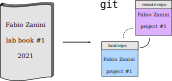
\includegraphics[width=0.8\linewidth]{git.pdf}
\caption{Git is the coding equivalent of lab books. However, each of your project has a separate "lab book", called a repository or ``repo''. It is common to have two copies of each repo, one local on your computer and one online that you can share with collaborators.}
\label{}
\end{center}
\end{figure}
In the lab, everyone keeps a lab book, a sort of professional diary that records each experiment conducted including its result, failures, successes, and changes from a previous iteration. Peeking back to a page from last year to check on an old protocol happens all the time. In computer coding, the record keeping role is kept by version control systems (VCS), the most popular being git (\url{https://git-scm.com/}). Instead of a single lab book, you keep a different git folder on your computer for each 
one of your projects. Each of these folders is called a \textit{repository} or just \textit{repo}. Unlike paper notebooks, you don't run out of pages so you can track a project for years in one place. People usually have two copies of each repository, a local one on their own computer (local repo) and a remote one online (remote repo) that they can share access with collaborators. Github (\url{https://github.com}), GitLab (\url{https://gitlab.com}), and Bitbucket (\url{https://bitbucket.org/}) are common choices of providers for remote repo space.

Git is not too easy to master but it is extremely useful -- imagine going to the wet lab without a lab book, it sounds almost criminal! Just hang in there and if you need a good guide, Pro Git (\url{https://git-scm.com/book/}) is freely available online. 
To install git \textit{git}, depending on your operating system:

\begin{itemize}
\item Linux: your package manager
\item OSX: homebrew (\url{https://brew.sh/} -- other options on the git website)
\item Windows: \url{https://git-scm.com/download/win}
\end{itemize}

To flip back to an earlier version of your code, you would typically use an additional software. Popular choices, depending on your operating system, are:

\begin{itemize}
\item Linux: gitg (\url{https://wiki.gnome.org/Apps/Gitg})
\item OSX and Windows: sourcetree (\url{https://www.sourcetreeapp.com/})
\end{itemize}

These are called ``git tree viewers'' or ``git history viewers'' and there are many alternatives online, all compatible with git, so feel free to search for the one you like best.

\subsection{The Python equivalent of\dots?}
Data science and in particular bioinformatics is full of little programs that you run in the command line. They are sometimes buggy or obscure, and often not flexible enough. Compared to a command line tools that uses only files as data structures, Python is a lot more flexible. Believe it or not, a command line call is actually a mini-script in a language called \href{https://www.gnu.org/software/bash/}{Bash} (usually), which is quite a bit less beginner-friendly than Python.

The good news is that there is often a Python equivalent of a certain command-line tool. Examples from bioinformatics:

\begin{itemize}
\item \href{https://github.com/samtools/samtools}{samtools}: \href{https://pysam.readthedocs.io/en/latest/}{pysam}
\item \texttt{samtools faidx}: \href{https://github.com/mdshw5/pyfaidx}{pyfaidx}
\item questionable \texttt{bigWig} scripts: \href{http://genome.ucsc.edu/goldenPath/help/bigWig.html}{pyBigWig}
\end{itemize}

The message here is that if you can have a tool wrapped in a nice Python function -- people call this an API --, that's often better than using the command-line tool directly.

\subsection{A little bit of uselessness}
While I tried to list some useful tools and practices in this book, there are also a few that appeared attractive to me as a the beginner explorer, but which I have learned with time to consider \textit{usually} useless. Of course, they can be useful in specific circumstances. Moreover, the authors of these tools are for sure amazing people, I just don't happen to like this particular thing. Here the list (you don't need to agree with me -- just my opinion):

\begin{itemize}
\item \textbf{3D plots:} computer screens and paper are 2D anyway.
\item \textbf{Circos plots:} ever wondered why books are square, not round?
\item \textbf{Rainbow heatmaps:} red stands out, everything else looks samey
\item \textbf{IDEs for data science:} including matlab and Rstudio. IDEs are great for software engineers though.
\item \textbf{Windows:} sorry folks: \url{http://www.over-yonder.net/~fullermd/rants/winstupid/1}
\end{itemize}

\section{Concluding remarks}
The goal of this book is to provide some guidance to beginners of this wonderful activity called data exploration. Personally, I have a lot of fun exploring data most of the time, even though it gets annoying at times. Over wet lab experimentation, data exploration has a big advantage: it's much faster \textit{provided you hone your skills}. No need to wait for cells to grow, for mice to breed, or even for those special tubes to arrive from another country. While speed is usually satisfying, it also means that most of the time your skills are the bottleneck between you and your paper. This can feel like a lot of pressure, so it is important to balance this additional pressure with free time activities that relax and recharge your nerves.

Have fun exploring and send me some feedback if you can!

\subsection*{The author}
I am a Senior Researcher at UNSW Sydney, Australia and head of the Data Driven Biomedicine lab: \url{http://fabilab.org}. I have been exploring, analysing, and generating data for a decade or so, especially on viral evolution, viral infections, and single cell transcriptomics. I was trained as a physicist and hated coding for years, until I had the luck of working with a talented data analyst who showed me it can be fun (he's a consultant now, not sure that's a good sign). I have been doing research in Italy, Germany, France, the US, and Australia.

\newpage
\tableofcontents

%%%%%%%%%%%%%%%%%%%%%%%%%%%%%%%%%%%%%%%%%%%%%%%%%%%%%%%%%%%%%%%%%%%%%%%%%
%\bibliographystyle{plain}
%\bibliography{}
%%%%%%%%%%%%%%%%%%%%%%%%%%%%%%%%%%%%%%%%%%%%%%%%%%%%%%%%%%%%%%%%%%%%%%%%%
\end{document}
%%%%%%%%%%%%%%%%%%%%%%%%%%%%%%%%%%%%%%%%%%%%%%%%%%%%%%%%%%%%%%%%%%%%%%%%%

